\documentclass[border=12pt]{standalone}
\def\pgfsysdriver{pgfsys-dvisvgm.def}
\usepackage[dvisvgm]{xcolor}
\usepackage{xeCJK}
\setCJKmainfont{HaranoAjiGothic-Regular.otf}[BoldFont=HaranoAjiGothic-Bold.otf]
\setCJKsansfont{HaranoAjiGothic-Regular.otf}[BoldFont=HaranoAjiGothic-Bold.otf]
\usepackage{amsmath,amssymb,tikz,lmodern}
\usetikzlibrary{arrows.meta,positioning,calc,fit,backgrounds}
\renewcommand{\familydefault}{\sfdefault}
\definecolor{ink}{HTML}{25322F}
\definecolor{green}{HTML}{246657}
\definecolor{tint}{HTML}{EEF4F0}
\definecolor{soft}{HTML}{C6D2CC}
\definecolor{muted}{HTML}{52615B}
\newif\ifJapanese
\newcommand{\Tx}[2]{\ifJapanese #1\else #2\fi}
\newcommand{\Eff}{\overline{\operatorname{Eff}}}
\newcommand{\heading}[3]{{\color{green}\bfseries #1\quad\Tx{#2}{#3}}\\[5pt]}
% A white rectangle makes the complete citation label clickable, including spaces.
\newcommand{\refurl}[2]{\special{dvisvgm:raw <a xlink:href="#1" target="_blank" rel="noopener noreferrer">}{\setlength{\fboxsep}{0pt}\colorbox{white}{\color{green}\underline{\strut #2}}}\special{dvisvgm:raw </a>}}
\newcommand{\refedge}[3]{\refurl{\csname source#1\endcsname\string##page=#2}{#3}}
\newcommand{\SF}[2]{\refedge{sf}{#1}{#2}}
% GitHub's file preview does not support PDF page fragments.
\newcommand{\LA}[2]{\refurl{\sourcela}{#2}}
\newcommand{\Sch}[2]{\refedge{sch}{#1}{#2}}
\newcommand{\PS}[2]{\refedge{ps}{#1}{#2}}
\tikzset{
 card/.style={draw=soft,fill=white,rounded corners=2pt,align=left,text=ink,font=\fontsize{10.5}{14}\selectfont,inner xsep=12pt,inner ysep=10pt,text width=14.4cm},
 half/.style={card,text width=6.45cm,minimum height=2.05cm},
 result/.style={card,draw=green,fill=tint,line width=.9pt},
 reason/.style={align=left,text=muted,font=\fontsize{9}{12}\selectfont,inner sep=0pt,text width=12.7cm},
 branchreason/.style={reason,text width=5.95cm},
 edge/.style={-{Stealth[length=2.4mm]},draw=green,line width=1pt},
 wire/.style={draw=green,line width=1pt},
}
% Keep the arrow in a dedicated left gutter; explanations never cover it.
\newcommand{\flow}[3]{
 \coordinate (#2-from) at ($(#1.south)+(-6.9,0)$);
 \coordinate (#2-to) at ($(#2.north)+(-6.9,0)$);
 \draw[edge] (#2-from)--(#2-to);
 \node[reason,anchor=west] (#2-reason) at ($(#2-from)!.5!(#2-to)+(.55,0)$) {#3};
}

\newcommand{\Hash}[2]{\refurl{\sourcehash}{#2}}
\newcommand{\FGring}[2]{\refedge{rings}{#1}{#2}}
\newcommand{\FGglue}[2]{\refedge{glue}{#1}{#2}}
\newcommand{\OI}[2]{\refurl{\sourceoi}{#2}}

\Japanesetrue
\newcommand{\sourcela}{https://github.com/openai/math/blob/adc7f1241b42e322a6451854ab7e4b4c146bf78a/preprints/Log-abundance-in-characteristic-zero-September-24-2026/paper.pdf}
\newcommand{\sourcehash}{https://arxiv.org/html/1609.00121v4}
\newcommand{\sourceglue}{https://www.math.kyoto-u.ac.jp/~fujino/fg-comp-final.pdf}
\newcommand{\sourcerings}{https://www.math.kyoto-u.ac.jp/~fujino/log-ring-aspm.pdf}
\newcommand{\sourceoi}{https://github.com/openai/math/blob/adc7f1241b42e322a6451854ab7e4b4c146bf78a/preprints/Orbifold-and-logarithmic-Iitaka-subadditivity-September-26-2026/paper.pdf}
\newcommand{\sourcehps}{https://people.math.harvard.edu/~mpopa/papers/HPS.pdf}
\newcommand{\sourcegmm}{https://github.com/openai/math/blob/adc7f1241b42e322a6451854ab7e4b4c146bf78a/preprints/Minimal-models-and-Mori-fibre-spaces-for-generalized-log-canonical-Q-pairs-September-24-2026/paper.pdf}
\begin{document}
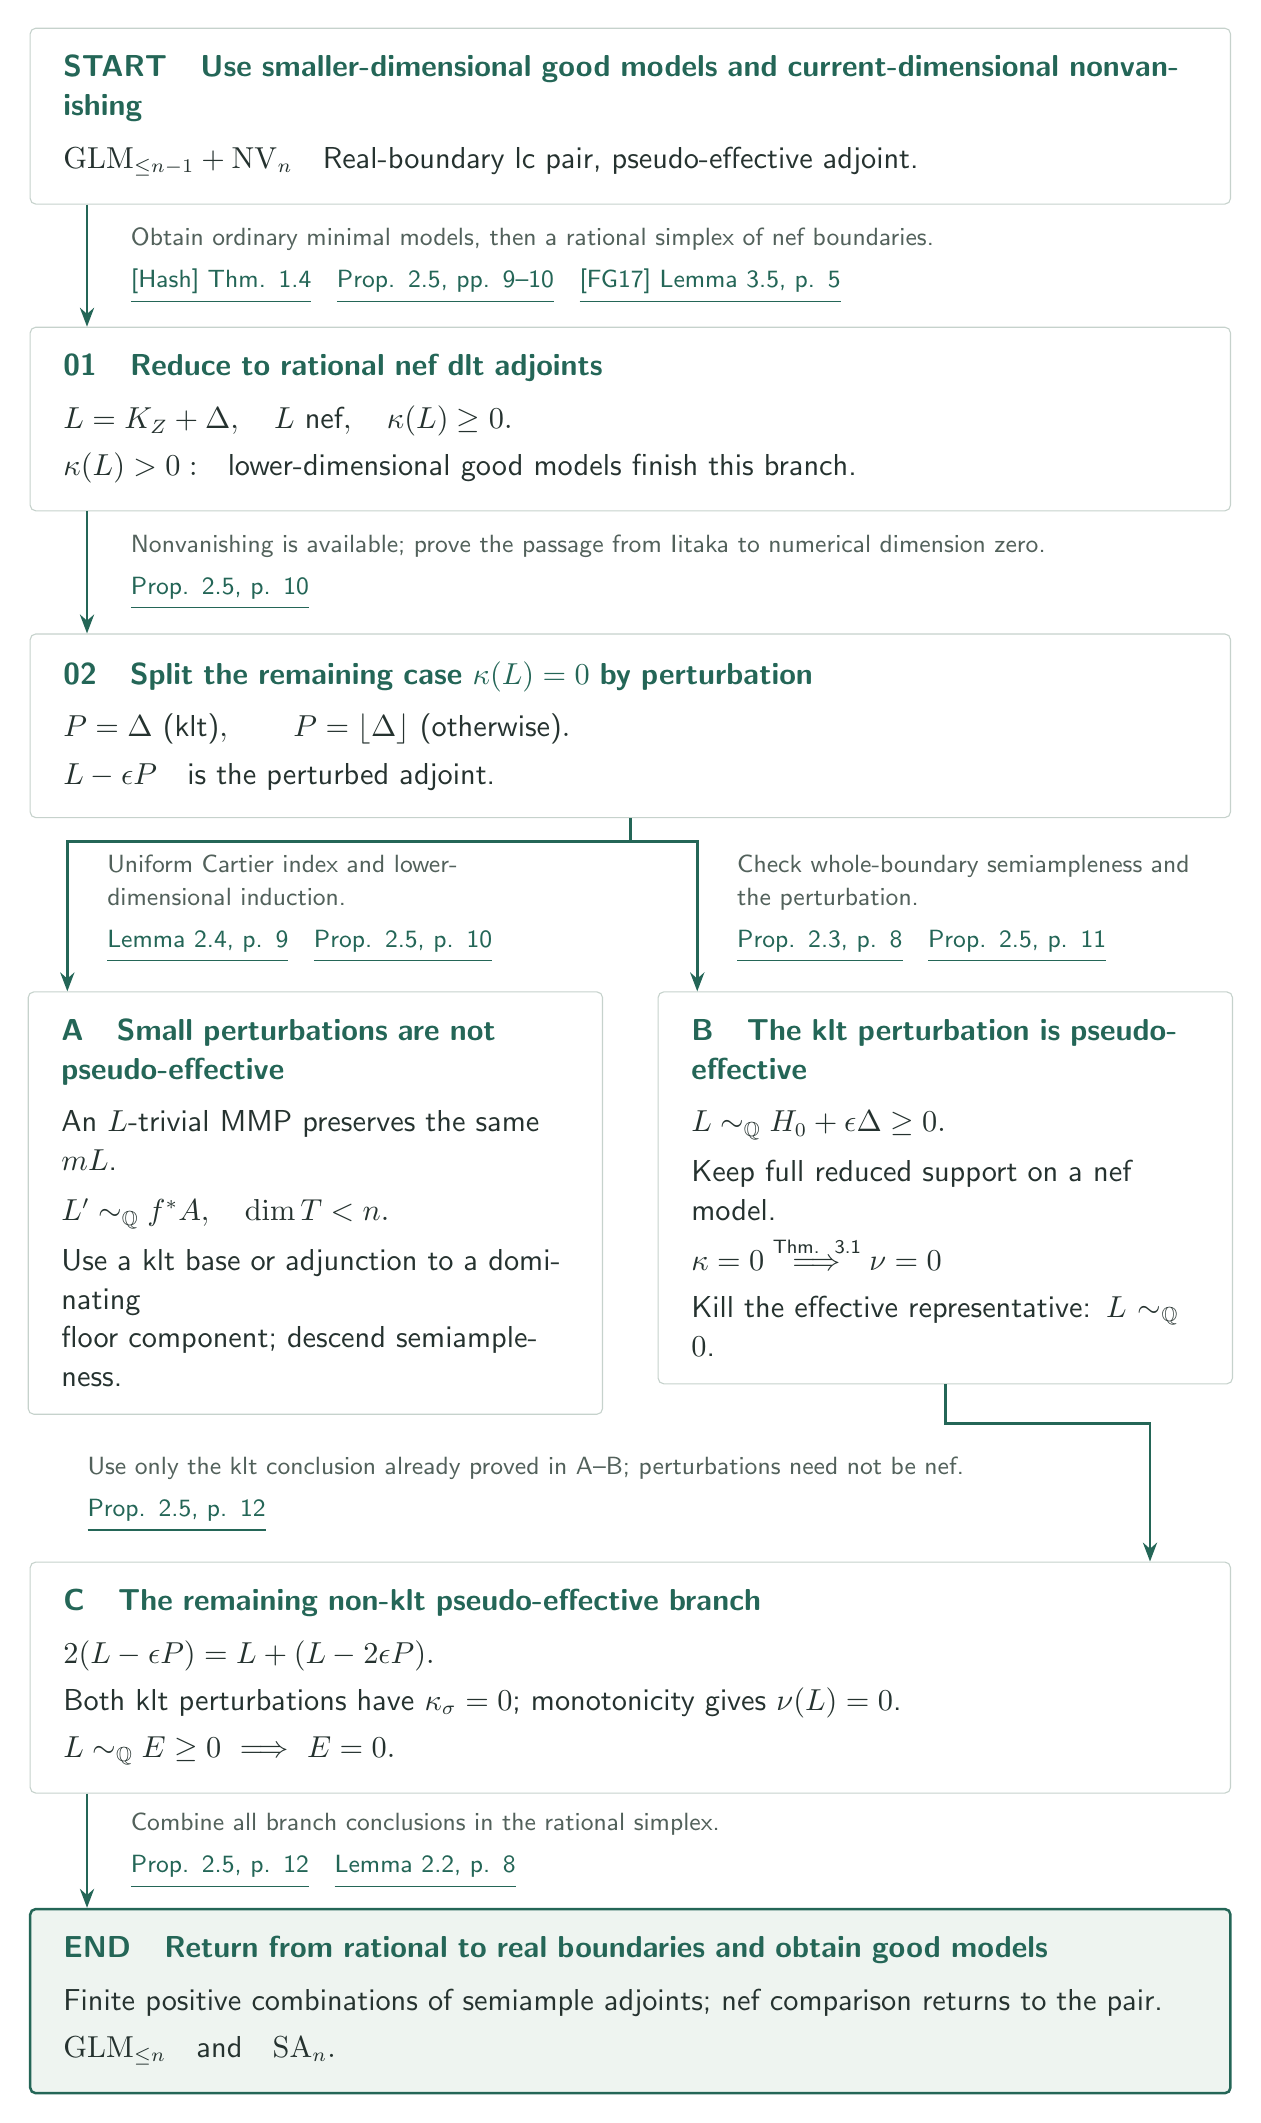
\begin{tikzpicture}
\node[card] (start) {\heading{START}{低次元の良いモデルと、同次元の非消滅を使う}{Use smaller-dimensional good models and current-dimensional nonvanishing}
$\mathrm{GLM}_{\leq n-1}+\mathrm{NV}_n$\quad\Tx{実係数 lc 対、随伴因子は擬有効。}{Real-boundary lc pair, pseudo-effective adjoint.}};
\node[card,below=1.55cm of start] (rational) {\heading{01}{有理係数の nef dlt 随伴因子へ}{Reduce to rational nef dlt adjoints}
$L=K_Z+\Delta,\quad L\text{ nef},\quad\kappa(L)\geq0.$\\[3pt]
$\kappa(L)>0:$\quad\Tx{低次元の良いモデルで完了。}{lower-dimensional good models finish this branch.}};
\flow{start}{rational}{\Tx{通常の極小モデルを得て、nef 境界の有理単体へ分解。}{Obtain ordinary minimal models, then a rational simplex of nef boundaries.}\\[3pt]\Hash{1}{[Hash] Thm. 1.4}\quad\LA{9}{Prop. 2.5, pp. 9--10}\quad\FGring{5}{[FG17] Lemma 3.5, p. 5}}
\node[card,below=1.55cm of rational] (zero) {\heading{02}{残る $\kappa(L)=0$ を摂動で分ける}{Split the remaining case $\kappa(L)=0$ by perturbation}
$P=\Delta\ \text{(klt)},\qquad P=\lfloor\Delta\rfloor\ \text{(otherwise)}.$\\[3pt]
$L-\epsilon P$\quad\Tx{の擬有効性を調べる。}{is the perturbed adjoint.}};
\flow{rational}{zero}{\Tx{非消滅は獲得済み。小平次元0から数値次元0への移行を証明する。}{Nonvanishing is available; prove the passage from Iitaka to numerical dimension zero.}\\[3pt]\LA{10}{Prop. 2.5, p. 10}}
\node[half,below=2.2cm of zero.south,anchor=north,xshift=-4cm,minimum height=3.3cm] (mori) {\heading{A}{小摂動が擬有効でない}{Small perturbations are not pseudo-effective}
\Tx{同じ $mL$ を保つ $L$-trivial MMP。}{An $L$-trivial MMP preserves the same $mL$.}\\[4pt]
$L'\sim_{\mathbb Q}f^*A,\quad\dim T<n.$\\[4pt]
\Tx{klt 底、または支配的な境界に随伴。\\半豊富性を底へ降ろす。}{Use a klt base or adjunction to a dominating\\floor component; descend semiampleness.}};
\node[half,below=2.2cm of zero.south,anchor=north,xshift=4cm,minimum height=3.3cm] (klt) {\heading{B}{klt で摂動が擬有効}{The klt perturbation is pseudo-effective}
$L\sim_{\mathbb Q}H_0+\epsilon\Delta\geq0.$\\[4pt]
\Tx{解消・nef モデルで全被約台を確保。}{Keep full reduced support on a nef model.}\\[4pt]
$\kappa=0\overset{\text{Thm. 3.1}}{\Longrightarrow}\nu=0$\\[3pt]
\Tx{有効代表元を消し、$L\sim_{\mathbb Q}0$。}{Kill the effective representative: $L\sim_{\mathbb Q}0$.}};
\draw[wire] (zero.south)--++(0,-.3) coordinate (fork);
\draw[edge] (fork)-| ($(mori.north)+(-3.15,0)$);
\draw[edge] (fork)-| ($(klt.north)+(-3.15,0)$);
\node[branchreason,anchor=west] at ($(mori.north)+(-2.65,1.05)$) {\Tx{Cartier 指数の一様性と低次元帰納。}{Uniform Cartier index and lower-dimensional induction.}\\[3pt]\LA{9}{Lemma 2.4, p. 9}\quad\LA{10}{Prop. 2.5, p. 10}};
\node[branchreason,anchor=west] at ($(klt.north)+(-2.65,1.05)$) {\Tx{全境界の半豊富性と小摂動を確認。}{Check whole-boundary semiampleness and the perturbation.}\\[3pt]\LA{8}{Prop. 2.3, p. 8}\quad\LA{11}{Prop. 2.5, p. 11}};
\node[card,below=2.25cm of klt.south,anchor=north,xshift=-4cm] (lc) {\heading{C}{残る非klt・擬有効の枝}{The remaining non-klt pseudo-effective branch}
$2(L-\epsilon P)=L+(L-2\epsilon P).$\\[3pt]
\Tx{二つの klt 摂動は $\kappa_\sigma=0$。単調性で $\nu(L)=0$。}{Both klt perturbations have $\kappa_\sigma=0$; monotonicity gives $\nu(L)=0$.}\\[3pt]
$L\sim_{\mathbb Q}E\geq0\ \Longrightarrow\ E=0.$};
\draw[edge] (klt.south)--++(0,-.5)-| ($(lc.north)+(6.6,0)$);
\node[reason,text width=12.8cm,anchor=west] at ($(lc.north)+(-6.9,.85)$) {\Tx{A・Bで証明済みの klt 結論だけを使う。摂動は nef と仮定しない。}{Use only the klt conclusion already proved in A--B; perturbations need not be nef.}\\[3pt]\LA{12}{Prop. 2.5, p. 12}};
\node[result,below=1.45cm of lc] (end) {\heading{END}{有理係数から実係数へ戻し、良いモデルを得る}{Return from rational to real boundaries and obtain good models}
\Tx{半豊富な有理随伴因子の有限正結合。元の nef 対へは比較で降下。}{Finite positive combinations of semiample adjoints; nef comparison returns to the pair.}\\[3pt]
$\mathrm{GLM}_{\leq n}\quad\text{and}\quad\mathrm{SA}_n.$};
\flow{lc}{end}{\Tx{全分岐の結論を有理単体へ戻す。}{Combine all branch conclusions in the rational simplex.}\\[3pt]\LA{12}{Prop. 2.5, p. 12}\quad\LA{8}{Lemma 2.2, p. 8}}
\end{tikzpicture}

\end{document}
